\section{Sets}

Sets provide the membership language used throughout the notes: elements, subsets, products, power sets, operations, and indexed families.

\subsection{Introduction to Sets}

\begin{definition} \label{def:sets-and-membership} \hlt{Sets and Membership}\\
Sets and the membership relation are taken as primitive notions.
\begin{enumerate}[label=(\roman*)]
\setlength{\itemsep}{0pt}
\item \hlt{Membership}: Given an object $x$ and a set $E$, the assertion $x\in E$ means that $x$ is an element of $E$; its negation is written $x\notin E$.
\item \hlt{Empty set}: The symbol $\emptyset$ denotes a set satisfying $x\notin\emptyset$ for every object $x$.
\end{enumerate}
\end{definition}

\begin{definition} \label{def:set-builder-notation} \hlt{Set-Builder Notation}\\
For a set $X$ and a condition $P(x)$ on its elements, $\{x\in X:P(x)\}$ denotes the set of all $x\in X$ satisfying $P(x)$.
\end{definition}


\subsection{Cartesian Products}

\begin{definition} \label{def:cartesian-product} \hlt{Ordered Pairs and Cartesian Products}\\
Coordinate order is part of both constructions.
\begin{enumerate}[label=(\roman*)]
\setlength{\itemsep}{0pt}
\item \hlt{Ordered pair}: For objects $a,b$, $(a,b)$ has first coordinate $a$ and second coordinate $b$.
\item \hlt{Equality}: For objects $a,b,a',b'$, $(a,b)=(a',b')$ if and only if $a=a'$ and $b=b'$.
\item \hlt{Cartesian product}: For sets $X$ and $Y$, $X\times Y\defeq\{(x,y):x\in X,\ y\in Y\}$.
\end{enumerate}
\end{definition}

For intervals $A$ and $B$, the Cartesian product $A\times B$ has a rectangular geometric representation.

\begin{illustrationfigure}[H]
    \centering
    \begin{tikzpicture}[
  >=Stealth,
  every node/.style={font=\small},
  axis/.style={->, gray!65, line width=0.45pt},
  interval/.style={line width=1.2pt},
  product/.style={draw=blue!60!black, fill=blue!8, line width=0.55pt},
  guide/.style={gray!55, dashed, line width=0.4pt},
  point/.style={circle, fill=black, inner sep=1.2pt}
]
  \draw[axis] (-0.25,0) -- (5.3,0);
  \draw[axis] (0,-0.25) -- (0,3.5);

  \coordinate (A0) at (1.15,0);
  \coordinate (A1) at (4.55,0);
  \coordinate (B0) at (0,0.8);
  \coordinate (B1) at (0,2.85);

  \draw[product] (1.15,0.8) rectangle (4.55,2.85);
  \draw[interval, blue!60!black] (A0) -- (A1);
  \draw[interval, orange!75!black] (B0) -- (B1);

  \node[below=5pt, blue!60!black] at (4.25,0) {$A$};
  \node[left=5pt, orange!75!black] at (0,2.75) {$B$};
  \node[blue!55!black, anchor=south east] at (4.35,0.92) {$A\times B$};

  \coordinate (P) at (2.75,2.05);
  \draw[guide] (2.75,0) -- (P);
  \draw[guide] (0,2.05) -- (P);
  \node[point] at (P) {};
  \node[below=1pt] at (2.75,0) {$a$};
  \node[left=2pt] at (0,2.05) {$b$};
  \node[above right=2pt] at (P) {$(a,b)$};
\end{tikzpicture}

    \caption{The product region $A\times B$ for horizontal interval $A$ and vertical interval $B$.}
    \label{fig:cartesian-product-rectangle}
\end{illustrationfigure}

Figure \ref{fig:cartesian-product-rectangle} illustrates Definition \ref{def:cartesian-product}: $(a,b)\in A\times B$ precisely when $a\in A$ and $b\in B$, in that order.


\subsection{Subsets and Power Sets}

\begin{definition} \label{def:proper-subsets-singletons-and-nonempty} \hlt{Basic Subset Terminology}\\
Let $A,B$ be sets.
\begin{enumerate}[label=(\roman*)]
\setlength{\itemsep}{0pt}
\item \hlt{Subset}: $A\subseteq B$ if and only if $x\in A$ implies $x\in B$ for every object $x$.
\item \hlt{Proper subset}: $A\subsetneq B$ iff $A\subseteq B$ and $A\neq B$.
\item \hlt{Singleton}: $A=\{x\}$ for some object $x$.
\item \hlt{Nonempty}: $A\neq\emptyset$.
\end{enumerate}
\end{definition}

\begin{assumption} \label{assump:set-extensionality} \hlt{Set Extensionality}\\
Throughout these notes, set equality is governed by extensionality.\\
For sets $A$ and $B$, $A=B$ if and only if $A\subseteq B$ and $B\subseteq A$.
\end{assumption}

\begin{proofmethod} \label{meth:proof-by-containment} \hlt{Proof by Two Containments}\\
To prove equality of sets $A$ and $B$, discharge the following obligations.
\begin{enumerate}[label=(\roman*)]
\setlength{\itemsep}{0pt}
\item Fix an arbitrary $x\in A$ and prove $x\in B$; this establishes $A\subseteq B$.
\item Fix an arbitrary $x\in B$ and prove $x\in A$; this establishes $B\subseteq A$.
\item Invoke Assumption \ref{assump:set-extensionality} to conclude $A=B$.
\end{enumerate}
If both sets have explicit membership criteria, the two inclusions may be proved together.\\
Fix an arbitrary object $x$ and prove $x\in A\Longleftrightarrow x\in B$.
\end{proofmethod}

\begin{definition} \label{def:power-set} \hlt{Power Set}\\
For a set $X$, its \hlt{power set} is $\mathcal{P}(X)\defeq\{S:S\subseteq X\}$.
The two smallest cases are as follows.
\begin{enumerate}[label=(\roman*)]
\setlength{\itemsep}{0pt}
\item The empty set has only itself as a subset, so $\mathcal{P}(\emptyset)=\{\emptyset\}$.
\item If $X=\{a,b\}$ with $a\neq b$, then $\mathcal{P}(X)=\{\emptyset,\{a\},\{b\},X\}$.
\end{enumerate}
\end{definition}


\subsection{Union, Intersection, Difference, and Complement}

\begin{definition} \label{def:analysis-sets-and-operations} \hlt{Elementary Set Operations}\\
Let $X$ be a set and let $A,B\subseteq X$.
\begin{enumerate}[label=(\roman*)]
\setlength{\itemsep}{0pt}
\item \hlt{Union}: $A\cup B\defeq\{x\in X:x\in A\text{ or }x\in B\}$.
\item \hlt{Intersection}: $A\cap B\defeq\{x\in X:x\in A\text{ and }x\in B\}$.
\item \hlt{Difference}: $A\setminus B\defeq\{x\in X:x\in A\text{ and }x\notin B\}$.
\item \hlt{Complement}: $A^c\defeq X\setminus A$, relative to the ambient set $X$.
\end{enumerate}
\end{definition}

\begin{definition} \label{def:symmetric-difference-of-events-and-sets} \hlt{Symmetric Difference}\\
Let $X$ be a set and let $A,B\subseteq X$.
The \hlt{symmetric difference} is $A\triangle B\defeq(A\setminus B)\cup(B\setminus A)$.\\
It consists exactly of the elements belonging to one of $A$ and $B$, but not both.
\end{definition}

\begin{proposition} \label{prop:analysis-set-algebra} \hlt{Basic Set Algebra}\\
Let $X$ be a set and let $A,B,C\subseteq X$. Then
\begin{enumerate}[label=(\roman*)]
\setlength{\itemsep}{0pt}
\item $A\cap(B\cup C)=(A\cap B)\cup(A\cap C)$;
\item $A\cup(B\cap C)=(A\cup B)\cap(A\cup C)$;
\item $(A\cup B)^c=A^c\cap B^c$;
\item $(A\cap B)^c=A^c\cup B^c$;
\item $A\triangle B=(A\cup B)\setminus(A\cap B)$.
\end{enumerate}
\begin{proof}
Fix an arbitrary $x\in X$.
By set extensionality, each identity follows once its two membership conditions are equivalent.
\begin{enumerate}[label=(\roman*)]
\setlength{\itemsep}{0pt}
\item[(i)] Membership in $A\cap(B\cup C)$ means that $x\in A$ and that either $x\in B$ or $x\in C$.
This holds exactly when either $x\in A\cap B$ or $x\in A\cap C$.
Hence it is equivalent to membership in $(A\cap B)\cup(A\cap C)$.
\item[(ii)] Membership in $A\cup(B\cap C)$ means that $x\in A$, or that both $x\in B$ and $x\in C$.
This holds exactly when two conditions are satisfied.
First, $x\in A$ or $x\in B$; second, $x\in A$ or $x\in C$.
Hence it is equivalent to membership in $(A\cup B)\cap(A\cup C)$.
\item[(iii)] The condition $x\in(A\cup B)^c$ is equivalent to $x\notin A\cup B$.
This means that $x\notin A$ and $x\notin B$, or equivalently $x\in A^c\cap B^c$.
\item[(iv)] The condition $x\in(A\cap B)^c$ is equivalent to $x\notin A\cap B$.
This means that $x\notin A$ or $x\notin B$, or equivalently $x\in A^c\cup B^c$.
\item[(v)] The condition $x\in A\triangle B$ is equivalent to $x\in A\setminus B$ or $x\in B\setminus A$.
Thus $x$ belongs to one of $A$ and $B$, but not both.
Equivalently, $x\in A\cup B$ and $x\notin A\cap B$.
By the definition of difference, this is equivalent to $x\in(A\cup B)\setminus(A\cap B)$.
\end{enumerate}
\hlt{Structural Commentary}: Each identity reduces to an equivalence of membership conditions.\\
\hlt{Key Insight}: Membership turns set operations into logical connectives.
\end{proof}
\end{proposition}

\begin{illustrationfigure}[H]
    \centering
    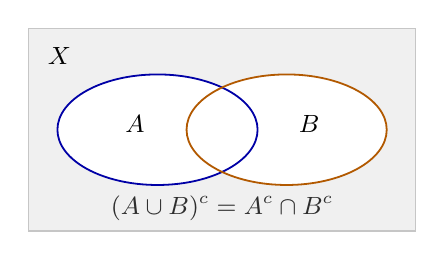
\begin{tikzpicture}[
  x=0.82cm,
  y=0.78cm,
  every node/.style={font=\small},
  ambient/.style={draw=gray!45, fill=gray!12, line width=0.5pt},
  setA/.style={draw=blue!65!black, line width=0.65pt},
  setB/.style={draw=orange!70!black, line width=0.65pt}
]
  \draw[ambient] (-3,-1.65) rectangle (3,1.65);
  \fill[white] (-1.0,0) ellipse (1.55 and 0.9);
  \fill[white] (1.0,0) ellipse (1.55 and 0.9);
  \draw[setA] (-1.0,0) ellipse (1.55 and 0.9);
  \draw[setB] (1.0,0) ellipse (1.55 and 0.9);

  \node at (-1.35,0.1) {$A$};
  \node at (1.35,0.1) {$B$};
  \node[anchor=north west] at (-2.85,1.5) {$X$};
  \node[gray!35!black] at (0,-1.28) {$(A\cup B)^c=A^c\cap B^c$};
\end{tikzpicture}

    \caption{The shaded region represents $(A\cup B)^c=A^c\cap B^c$ inside the ambient set $X$.}
    \label{fig:de-morgan-complement-union}
\end{illustrationfigure}

Figure \ref{fig:de-morgan-complement-union} illustrates part (iii).
The shaded region lies outside both $A$ and $B$, so it is outside $A\cup B$.


\subsection{Indexed Families and Products}

\begin{definition} \label{def:indexed-families-unions-intersections} \hlt{Families, Indexed Families, Unions, and Intersections}\\
Let $X$ be a set and let $I$ be an index set.
\begin{enumerate}[label=(\roman*)]
\setlength{\itemsep}{0pt}
\item \hlt{Family}: A set whose members are sets, also called a \hlt{collection} of sets.
\item \hlt{Indexed family}: An assignment $i\mapsto A_i$ over $I$, written $(A_i)_{i\in I}$ or $\{A_i\}_{i\in I}$.
It is an indexed family in $X$ iff $(\forall i\in I)\,A_i\subseteq X$.
\item \hlt{Indexed union}: For an indexed family $\{A_i\}_{i\in I}$ in $X$, $\bigcup\limits_{i\in I}A_i\defeq\{x\in X:(\exists i\in I)\,x\in A_i\}$.
\item \hlt{Indexed intersection}: For an indexed family $\{A_i\}_{i\in I}$ in $X$, $\bigcap\limits_{i\in I}A_i\defeq\{x\in X:(\forall i\in I)\,x\in A_i\}$.
\end{enumerate}
\end{definition}

\begin{theorem} \label{thm:indexed-de-morgan-laws} \hlt{Arbitrary De Morgan Laws}\\
Let $X$ and $I$ be sets, and let $\{E_i\}_{i\in I}$ be an indexed family in $X$.
Take all complements relative to $X$.
\begin{enumerate}[label=(\roman*)]
\setlength{\itemsep}{0pt}
\item $\left(\bigcup\limits_{i\in I}E_i\right)^c=\bigcap\limits_{i\in I}E_i^c$.
\item $\left(\bigcap\limits_{i\in I}E_i\right)^c=\bigcup\limits_{i\in I}E_i^c$.
\end{enumerate}
\begin{proof}
Fix an arbitrary $x\in X$.
Extensionality reduces both identities to pointwise membership equivalences.
\begin{enumerate}[label=(\roman*)]
\setlength{\itemsep}{0pt}
\item $x\in\left(\bigcup\limits_{i\in I}E_i\right)^c\iff(\forall i\in I)\,x\notin E_i\iff(\forall i\in I)\,x\in E_i^c\iff x\in\bigcap\limits_{i\in I}E_i^c$.
\item $x\in\left(\bigcap\limits_{i\in I}E_i\right)^c\iff(\exists i\in I)\,x\notin E_i\iff(\exists i\in I)\,x\in E_i^c\iff x\in\bigcup\limits_{i\in I}E_i^c$.
\end{enumerate}
\hlt{Structural Commentary}: The proof checks both identities pointwise and applies quantifier negation.\\
\hlt{Key Insight}: Complement exchanges existential and universal membership conditions.
\end{proof}
\end{theorem}

\begin{definition} \label{def:disjoint-families-and-parametrizations} \hlt{Disjoint Families and Parametrizations}\\
Let $I$ be an index set and let $\mathcal{F}$ be a family of sets.
Let $\{A_i\}_{i\in I}$ be an indexed family of sets.
\begin{enumerate}[label=(\roman*)]
\setlength{\itemsep}{0pt}
\item \hlt{Pairwise disjoint}: $(\forall E,G\in\mathcal{F})\,(E\neq G\implies E\cap G=\emptyset)$.
\item \hlt{Parametrization}: $\{A_i\}_{i\in I}$ parametrizes $\mathcal{F}$ iff $\mathcal{F}=\{A_i:i\in I\}$.
\end{enumerate}
\end{definition}

\begin{definition} \label{def:indexed-cartesian-product} \hlt{Cartesian Product of an Indexed Family}\\
Let $I$ be an index set and let $\{E_i\}_{i\in I}$ be an indexed family of sets.
\begin{enumerate}[label=(\roman*)]
\setlength{\itemsep}{0pt}
\item \hlt{Product}: $\prod\limits_{i\in I}E_i\defeq\{(x_i)_{i\in I}:(\forall i\in I)\,x_i\in E_i\}$.
\item \hlt{Binary case}: If $I=\{1,2\}$, identify $(x_i)_{i\in I}$ with the ordered pair $(x_1,x_2)$.
Under this identification, $\prod\limits_{i\in I}E_i=E_1\times E_2$.
\item \hlt{Constant family}: If $E$ is a set and $(\forall i\in I)\,E_i=E$, write $E^I\defeq\prod\limits_{i\in I}E_i$.
Thus $E^I$ is the set of $I$-indexed families in $E$.
\item \hlt{Dependence}: Different parametrizations of the same family can yield different products.
\end{enumerate}
\end{definition}


\subsection{Russell's Paradox and Axioms}

\begin{theorem} \label{thm:russells-paradox} \hlt{Russell's Paradox}\\
For a condition $P(x)$ on sets, unrestricted comprehension asserts $(\exists R)(\forall x)\,[x\in R\Longleftrightarrow P(x)]$.
\begin{enumerate}[label=(\roman*)]
\setlength{\itemsep}{0pt}
\item No set $R$ satisfies $(\forall x)\,[x\in R\Longleftrightarrow x\notin x]$.
\item The unrestricted comprehension schema is inconsistent.
\end{enumerate}
\begin{proof}
\begin{enumerate}[label=(\roman*)]
\setlength{\itemsep}{0pt}
\item Suppose that such a set $R$ exists. Setting $x=R$ gives $R\in R\Longleftrightarrow R\notin R$. If $R\in R$, then $R\notin R$; if $R\notin R$, then $R\in R$.\\
Both cases are contradictory, so no such set exists.
\item Take $P(x)\defeq x\notin x$.
The corresponding instance asserts
$(\exists R)(\forall x)\,[x\in R\Longleftrightarrow x\notin x]$.
This contradicts (i), proving (ii).
\end{enumerate}
\hlt{Structural Commentary}: Specialize at $x=R$, then apply the matching comprehension instance.\\
\hlt{Key Insight}: Self-membership makes the defining condition assert its own negation.
\end{proof}
\end{theorem}

\begin{perspective} \label{per:zfc-axiom-role-map} \hlt{From Comprehension to Axioms}\\
The obstruction in Theorem \ref{thm:russells-paradox} explains the need for controlled set formation.\\
Separation forms $\{x\in B:P(x)\}$ only after a bounding set $B$ is available.
The standard ZFC axioms have the following informal roles.
\begin{enumerate}[label=(\roman*)]
\setlength{\itemsep}{0pt}
\item \hlt{Extensionality} makes membership determine set equality.
\item \hlt{Separation} extracts a condition-defined subset from an existing bounding set.
\item \hlt{Pairing} supplies $\{a,b\}$ from given sets $a$ and $b$, including $\{a\}$ when $a=b$.
\item \hlt{Union} collects into one set the elements of the members of a given set.
\item \hlt{Power set} supplies $\mathcal{P}(A)$, the set of all subsets of a given set $A$.
\item \hlt{Infinity} supplies an inductive set from which the natural numbers are constructed.
\item \hlt{Replacement} forms the image of a set under a definable functional relation.
\item \hlt{Foundation} requires nonempty sets to contain an $\in$-minimal member.
\item \hlt{Choice} supplies a choice function on a set-indexed family of nonempty sets.
\end{enumerate}
This perspective is a functional map, not a formal axiom list or a source of proof authority.\\
Formal statements and dependencies belong to the advanced set-theory section.
\end{perspective}

